%%%%%%%%%%%%%%%%%%%%%%%%%%%%%%%%%%%%%%%%%%%%%%%%%%%%%%%%%%%%%%%%
% %
% Due Date %
% Andrew Gibson %
% ECE 351 lab, Section 53 %
% Lab 6 %
% Due 28 Feb 2023 %
% Step and Impulse Response of an RLC Bandpass Filter %
%https://github.com/gibs0630/ECE351\_Code %
%https://github.com/gibs0630/ECE351\_Reports %
% %
%%%%%%%%%%%%%%%%%%%%%%%%%%%%%%%%%%%%%%%%%%%%%%%%%%%%%%%%%%%%%%%%

\documentclass[12pt,a4paper]{article}
\usepackage[utf8]{inputenc}
\usepackage[greek,english]{babel}
\usepackage{alphabeta} 
\usepackage[pdftex]{graphicx}
\usepackage[top=1in, bottom=1in, left=1in, right=1in]{geometry}
\linespread{1.06}
\setlength{\parskip}{8pt plus2pt minus2pt}
\widowpenalty 10000
\clubpenalty 10000
\newcommand{\eat}[1]{}
\newcommand{\HRule}{\rule{\linewidth}{0.5mm}}
\usepackage[official]{eurosym}
\usepackage{enumitem}
\setlist{nolistsep,noitemsep}
\usepackage[hidelinks]{hyperref}
\usepackage{cite}
\usepackage{lipsum}

\newcommand{\Q}{\leavevmode\par\textbf {Q:}}
\newcommand{\A}{\par\textbf{A:} \normalfont}

\hypersetup{colorlinks=true, linkcolor=black, urlcolor=blue}

\begin{document}
%===========================================================
\begin{titlepage}
\begin{center}
% Top 
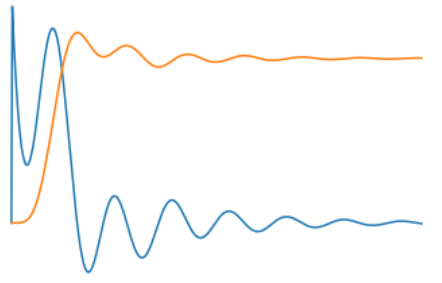
\includegraphics[width=0.55\textwidth]{titlepage_image.png}~\\[2cm]
% Title
\HRule \\[0.4cm]
{ \LARGE 
  \textbf{Project Report for ECE 351}\\[0.4cm]
  \emph{Lab 6: Partial Fraction Expansion}\\[0.4cm]
}
\HRule \\[1.5cm]
% Author
{ \large
  Andrew Gibson \\[0.1cm]
 21 February 2023\\[0.1cm]
  \url{https://github.com/gibs0630/ECE351\_Code}\\[0.1cm]
  \url{https://github.com/gibs0630/ECE351\_Reports}\\[0.1cm]
  %#\texttt{user@cut.ac.cy}
}
\vfill
%\textsc{\Large Cyprus University of Technology}\\[0.4cm]\textsc{\large Department of Electrical Engineering,\\Computer Engineering \& Informatics}\\[0.4cm]
% Bottom
{\large }
 
\end{center}
\end{titlepage}
%\begin{abstract}
%\lipsum[1-2]
%\addtocontents{toc}{\protect\thispagestyle{empty}}
%\end{abstract}
\newpage
%===========================================================
\tableofcontents
\addtocontents{toc}{\protect\thispagestyle{empty}}
\newpage
\setcounter{page}{1}
%===========================================================
%===========================================================
\section{Introduction}\label{sec:intro}
With a linear differential equation that is complex or has many many terms, it is most likely easier to solve using Laplace Transforms.
However, one of the key algebraic actions in the process is partial fraction expansion.  once the terms are expanded, it is then trivial to inverse Laplace back, even if there are complex values. Using signal synthesizer software these can be done automatically to find a signal's output after going through a complex system.

\section{Equations}\label{sec:lit-rev}
Formula's used
unit step function
\[
u(x) = \left\{
        \begin{array}{ll}
            0 & \quad t < 0 \\
            1 & \quad t \geq 0
        \end{array}
    \right.
\]

complex inverse Laplace

\[\mathcal{L} ^{-1}\left \lbrace \frac {\left(| k | \angle {k}\right)}{s+\left(\alpha+j\omega\right)} \right \rbrace = 2 |k| e^{\alpha t} cos(\omega t + \angle k ) u(t)\]

equations from the lab
\[y^{\prime \prime}(t) + 10y^{\prime}(t) + 24y(t) = x^{\prime\prime}(t) + 6x^{\prime}(t) + 12x(t) \]

\[y^{(5)}(t) + 18y^{(4)}(t) + 218y^{(3)}(t) + 2036y^{(2)}(t) + 9085y^{(1)}(t) + 25250y(t) = 25250x(t)\]

\section{Methodology}\label{sec:meth}
This lab had us analyze differential equations via hand calculations and then create a model in python to compare them.

\section{Results}\label{sec:res}
\subsection*{Part 1}

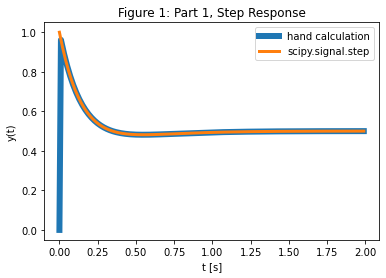
\includegraphics[width=0.55\textwidth]{Figure1.png}\\
The purpose producing Figure 1 to show that the step response from the hand calculation was the same as the computed  using the step function from the library skipy.


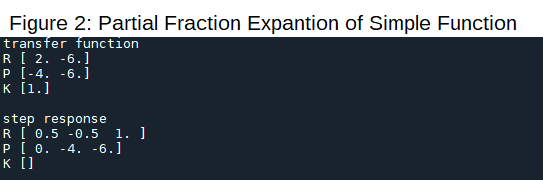
\includegraphics[width=0.55\textwidth]{Figure2.png}\\
Figure 2 is the Partial Fraction Expansion output from the transfer function and step response using the residue function from the library skipy.\\

\subsection*{Part 2}

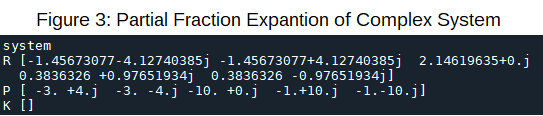
\includegraphics[width=0.55\textwidth]{Figure3.png}\\
Figure 3 is the Partial Fraction Expansion output complex system using the residue function from the library skipy.  of note there are complex values for the poles (offset to the s in the denominator)and for the residue (numerator in s-space)\\

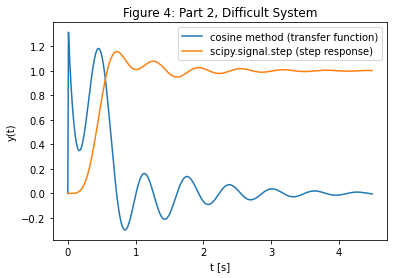
\includegraphics[width=0.55\textwidth]{Figure4.png}\\
Figure 2 shows the cosine method computed from using complex terms from a partial fraction expansion.  The step response would be the integral, of the transfer function, and that appears to be correct.\\



\section{Questions}\label{sec:res}


\Q 1. For a non-complex pole-residue term, you can still use the cosine method, explain why this works. 
\A 1. You can still use the cosine method because when both the numerator and denominator of the terms, ``$a / (s+b)$'', are in the real domain, then the angular frequency and angular displacement are 0. cosine of 0 is 1, which then harmlessly removes the term and we end up with out when the expected  ``$a*e^{-bt}$'' equation.


\Q 2. Leave any feedback on the clarity of the expectations, instructions, and  deliverables.
\A 2. The provided book does not list a complete exhaustive list of identities that can be used to derive laplaces and their inverses, however there was a clear confusion in the idenitying what term is laplaced in the "The Cosine  Method" section of the book as compared to the 4.3 task 3 of the lab.  If there was a formula written out for accepting complex roots in isolation  compared to when paired up with their complement, it woudl be easier to understand.



%\lipsum[7-8]\cite{knuthwebsite}
%===========================================================
%===========================================================
\bibliographystyle{ieeetr}
\bibliography{refs}
\end{document} 
Annotations











